%\VignetteIndexEntry{Using ssPATHS}
\documentclass{article}

\title{ssPATHS: Single Sample  PATHway Score (version 0.1.0)}
\date{2019\\ July}
\author{Natalie R. Davidson, Philipp Markolin, Gunnar R{\"a}tsch
        \\ Biomedical Informatics, ETH Z{\"u}rich}

\usepackage{Sweave}
\begin{document}
\maketitle


\Sconcordance{concordance:ssPATHS.tex:ssPATHS.Rnw:%
1 8 1 1 0 12 1 1 7 13 1 1 3 1 0 6 1 3 0 1 2 1 1 1 3 4 %
0 1 2 3 1 1 2 20 0 1 2 4 1 1 3 1 0 2 1 3 0 1 2 7 1 1 %
3 1 0 3 1 3 0 1 2 3 1 1 3 1 0 2 1 3 0 1 2 1 1 1 3 1 0 %
1 3 1 0 1 1 1 3 5 0 1 2 1 4 2 0 1 1 1 2 5 0 1 2 3 1 1 %
2 1 0 2 1 18 0 1 2 6 1 1 17 15 0 2 1 4 0 1 2 10 1}



\DefineVerbatimEnvironment{Sinput}{Verbatim} {xleftmargin=2em}
\DefineVerbatimEnvironment{Soutput}{Verbatim}{xleftmargin=2em}
\DefineVerbatimEnvironment{Scode}{Verbatim}{xleftmargin=2em}
\fvset{listparameters={\setlength{\topsep}{0pt}}}
\renewenvironment{Schunk}{\vspace{\topsep}}{\vspace{\topsep}}


\section{Introduction}

Precision oncology requires that a single patient can be accurately and
meaningfully characterized in order to tailor treatments.
Using our method, ssPATHS, we are able to estimate pathway
deviations for a single patient, by first learning a discriminative gene
weighting from a reference cohort. In this vignette, we use TCGA gene expression
data to learn a weighting on hypoxia-related genes then apply it to pancreatic
cancer cell lines to estimate the level of hypoxia within each sample.

\section{Formatting Data}

First, we load the appropriate packages we will need.
\begin{Schunk}
\begin{Sinput}
> library("dml")
> library("data.table")
> library("ROCR")
> library("MESS")
> library("ggplot2")
> library("ssPATHS")
> library("plyr")
\end{Sinput}
\end{Schunk}

Next, we will read in the TCGA data and format it appropriately.
\begin{Schunk}
\begin{Sinput}
> data(tcga_expr_df)
\end{Sinput}
\end{Schunk}

Let's look at the format of our data. To learn our gene weights we will need a
\emph{Y} column and a \emph{sample\_id} column.

\begin{Schunk}
\begin{Sinput}
> tcga_expr_df[1:6,1:5]
\end{Sinput}
\begin{Soutput}
                       tcga_id study is_normal
1 TCGA-CQ-6224-01A-11R-1915-07  HNSC     FALSE
2 TCGA-TQ-A7RP-01A-21R-A34F-07   LGG     FALSE
3 TCGA-13-1510-01A-02R-1565-13    OV     FALSE
4 TCGA-HC-8265-01A-11R-2263-07  PRAD     FALSE
5 TCGA-HC-7079-01A-11R-1965-07  PRAD     FALSE
6 TCGA-4X-A9FC-01A-11R-A42C-07  THYM     FALSE
  libsize_75percent ENSG00000078369
1         0.5201350       146190.89
2         0.4887488       105250.39
3         0.5159627        58773.63
4         0.3658994       101336.60
5         0.4617693        81393.47
6         0.3735174       101473.18
\end{Soutput}
\end{Schunk}

Since we are interested in hypoxia, we want to learn a weighting only on genes
associated with hypoxia. In this package we have a helper function to retreive
these genes, but other gene sets can be used for different pathways of interest.
Gene sets can be easily fetched using the package \emph{msigdbr}.
\begin{Schunk}
\begin{Sinput}
> hypoxia_gene_ids = get_hypoxia_genes()
> hypoxia_gene_ids = intersect(hypoxia_gene_ids, colnames(tcga_expr_df))
> hypoxia_df = tcga_expr_df[,c("tcga_id", "is_normal", hypoxia_gene_ids)]
\end{Sinput}
\end{Schunk}


Now we will need to identify how we want to discriminate our samples. Here, we
use the assumption that normal samples are less hypoxic than tumor samples.
Therefore, we will use the \emph{is\_normal} column as our \emph{Y} column.
We set normal samples to 0 and tumor samples to 1. This implies that a higher
score indicates a more hypoxic sample.

\begin{Schunk}
\begin{Sinput}
> colnames(hypoxia_df)[1:2] = c("sample_id", "Y")
> hypoxia_df$Y = 0
> hypoxia_df$Y[tcga_expr_df$is_normal==TRUE] = 0
> hypoxia_df$Y[tcga_expr_df$is_normal==FALSE] = 1
\end{Sinput}
\end{Schunk}

\section{Get Reference Gene Weightings }

Now that our data is in the appropriate format, we can learn the weightings.
\begin{Schunk}
\begin{Sinput}
> res = get_gene_weights(hypoxia_df)
> gene_weights = res[[1]]
> sample_scores = res[[2]]
\end{Sinput}
\end{Schunk}

Now let's see how well we did in seperating the two classes defined by \emph{Y}.
\begin{Schunk}
\begin{Sinput}
> training_res = get_classification_accuracy(sample_scores, positive_val=1)
> # plot the ROC curve
> plot(training_res[[4]], col="blue", ylim=c(0, 1))
> roc_text = paste("AUC:", round(training_res$auc_roc,3))
> legend(0.1,0.8, roc_text,
        border="white",cex=1,box.col = "white")
\end{Sinput}
\end{Schunk}
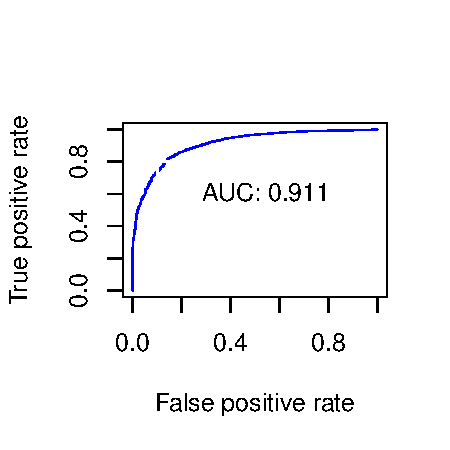
\includegraphics{ssPATHS-009}

\begin{Schunk}
\begin{Sinput}
> # plot the PR curve
> plot(training_res[[3]], col="orange", ylim=c(0, 1))
> pr_text = paste("AUC:", round(training_res$auc_pr,3))
> legend(0.1,0.8, pr_text,
        border="white",cex=1,box.col = "white")
\end{Sinput}
\end{Schunk}
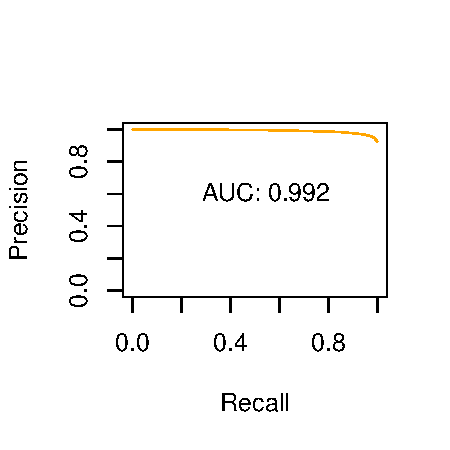
\includegraphics{ssPATHS-010}

\section{Apply Gene Weightings to New Samples}
Now, using the gene weightings learned from the reference set, we can apply
it to a new sample.
\begin{Schunk}
\begin{Sinput}
> data(new_samp_df)
> new_score_df = get_new_samp_score(gene_weights, new_samp_df)
> new_score_df
\end{Sinput}
\begin{Soutput}
          sample_id pathway_score
9   exp_norm_ctrl_C   -0.64176821
7   exp_norm_ctrl_A   -0.62781700
8   exp_norm_ctrl_B   -0.57268638
12 exp_norm_noHIF_C   -0.52251848
10 exp_norm_noHIF_A   -0.52041674
4   exp_hyp_noHIF_A   -0.50703636
5   exp_hyp_noHIF_B   -0.44738709
11 exp_norm_noHIF_B   -0.35926202
6   exp_hyp_noHIF_C   -0.31590814
3    exp_hyp_ctrl_C   -0.04498432
1    exp_hyp_ctrl_A   -0.02130225
2    exp_hyp_ctrl_B    0.12366948
\end{Soutput}
\end{Schunk}

Now lets see if the derived score match our experimental expectations.
Samples with \textbf{hyp} or \textbf{norm} in the sample id are cell lines
that were exposed to hypoxic or normoxic conditions respectively.
Samples with \textbf{ctrl} or \textbf{noHIF} were samples that were able to
produce a HIF-mediated hypoxic response or not, respectively.

\begin{Schunk}
\begin{Sinput}
> plot_scores <- function(hif_scores){
 
     # format the sample IDS
     hif_scores$sample_type = substr(hif_scores$sample_id, 1,
                                   nchar((hif_scores$sample_id))-2)
     colnames(hif_scores)[2] = "pathway_score"
 
     gg = ggplot(hif_scores, aes(x=sample_type, y=pathway_score,
                                   fill=sample_type)) +
         geom_boxplot() +
         theme(axis.text.x = element_text(angle = 90, hjust = 1)) +
         theme_bw()
 
         return(gg)
 }
> gg = plot_scores(new_score_df)
> print(gg)
\end{Sinput}
\end{Schunk}
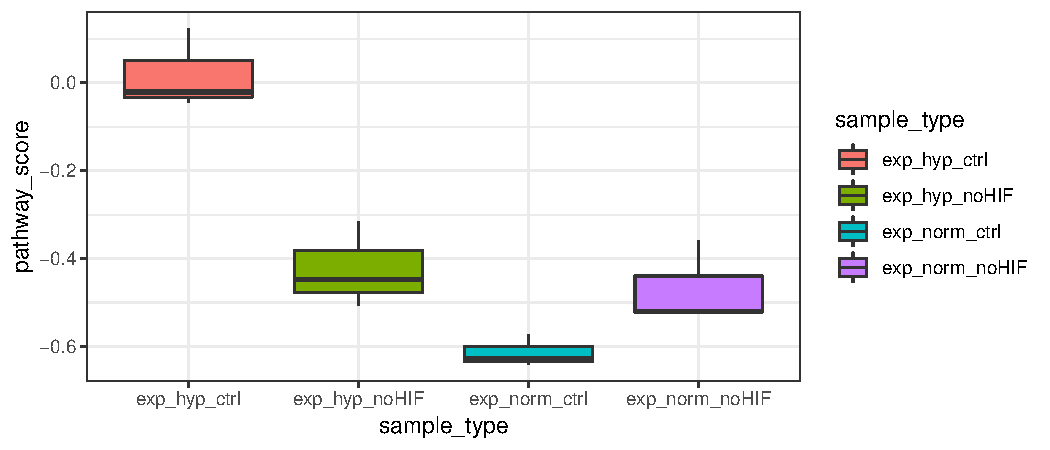
\includegraphics{ssPATHS-012}

Accordingly, we find the the \textbf{hyp\_ctrl} samples have the highest pathway
score. According to our labeling (tumor/hypoxic is 1 and normal/normoxic is 0),
this implies that these samples are the most hypoxic. Furthermore, we see that
the samples that were not able to produce a hypoxic response, even in the
absence of oxygen (\textbf{hyp\_noHIF}) are found to have similar score to the
normoxic samples.



\end{document}
